\chapter{Building a Topic Model}
\label{ch:building}

Previous chapters have focused on \emph{existing} models.  This
chapter focuses on how a researcher can create, implement, and
validate a new model.  We have described
models that researchers have created to capture particular nuances or
processes that exist in the world, but omit blueprints
for research who want to extend an existing model or create their own.

Before going into the details of constructing new models, we encourage users to consider whether questions can be answered through post-hoc analysis of a simple topic model in the context of additional information.
For example, a simple dynamic topic model can be constructed from a standard LDA model by slicing the corpus into sections and estimating the probability distribution over words for each topic in each section.
Building and validating custom topic models is a powerful tool, but requires significant investment in coding and debugging, and may not be able to take advantage of computational optimizations available for simpler models.
Posterior predictive checks \cite{mimno-11Bayesian} provide a good means of determining whether LDA topics or words within topics already show patterns that are present but not explicitly modeled.

It is impossible to cover all of the details of research in topic
models or machine learning generally, but this chapter introduces some
of the common techniques for creating new models.  We will focus on a
running example, creating a new model for predicting the
ideology of a political speaker.

\section{Designing a Model}

The first step in creating a new model is to define what is
important.  For example, previous chapters have focused on measuring
innovation, cross-language connections, and sentiment.  These are
high-level concepts that we want do discover from text.  We believe
these properties exist in the world, but we want the variables of our models to represent
these concepts.

In a topic model, incorporating a new concept into the model usually
involves adding a new random variable to the model.  This is where
intuitions and domain knowledge come to the forefront.  Because the
generative process attempts to model the real world, a new model must
balance several components that are often in tension: fidelity,
performance, tractability, and interpretability.

\paragraph{Fidelity}

A good model should reflect the world.  If political scientists
believe that a politician's ideology is a property that changes how they speak, then the model should place a
speaker's ideology upstream of the language politicians produce
(upstream vs. downstream models are discussed in \citet{mimno-08} and Chapter~\ref{ch:css}).

Modeling reality is a good idea. But just as building a scale model of a building requires compromises in terms of materials and level of detail, building a statistical model requires unreal assumptions.
If a generative model exactly
matches the process that produces data, we can prove that it will
converge to the correct answer~\citep{neal-93}.
But humans and text are
not Dirichlet and discrete distributions; all models are going to
be an approximation.

In addition to determining \emph{where} to model a feature in a
generative model, it is also important to decide \emph{how} to model
it.  Is it a continuous value, a binary value, a member of a discrete
set, or something else?  Often, we have multiple pre-defined notions of how to
represent a quantity of interest.
Sentiment is sometimes represented as a continuous positive or negative value, while review corpora include discrete, positive star ratings.
Political ideology could be represented by membership in one of a fixed number of
parties, but political scientists more often assign a continuous value to a
politician's ideology.

\paragraph{Performance}

Greater fidelity to our perceptions of how the world works does not always imply that models will be more  useful.
We sometimes have to trade off fidelity with performance.
Recent work seems to agree that \emph{downstream} models work better even though it is
less realistic~\citep{nguyen-13:shlda}.\footnote{One might argue that it is more realistic for
  a \emph{listener} who must interpret speech to assign an ideology
  after it has been heard, but this is no longer consistent with how
  the text was \emph{generated}.} 

It is nearly impossible to know \textit{a priori} whether a
model will work well for a particular task given just the model.
Knowing what will work best is often a trial-and-error
process.
However, it is often possible to draw parallels from similar models.
Upstream models allow metadata variables to better predict which topics
will occur in a context, but they do not necessarily encourage the model to 
learn different topics than a model without metadata.
Downstream models must align topics to best predict a metadata variable, 
and therefore tend to find different (but not necessarily better) topics.
Supervised topic models have therefore worked well for predicting sentiment as a downstream variable, so it might be reasonable to assume
that a downstream model would work well for ideology as well.

\paragraph{Tractability}

Now that we know what variable we want to model, some approaches to model that
variable could be easier than others.  Political ideology is often
thought of as a \emph{spectrum} rather than a label: some politicians
are more centrist than others even though they might have the same
party label.

However, discrete labels are appealing from a modeling perspective.
Dirichlet-discrete distributions (Chapter~\ref{ch:intro})
are easy to to combine.  Given that basic topic models are built from
Dirichlets and discrete distributions, it is easier to add an additional
Dirichlet-discrete than to add a continuous random variable to the
model.  For example, the Topic-Aspect model~\citep{paul-10} is far simpler to
implement than Supervised Topic Models~\citep{blei-07b}.

Dirichlets and discrete distributions play well together because they are
conjugate, while Gaussian distributions add additional
difficulty.  However, Gaussian distributions are more convenient than
other distributions.  For example, spherical distributions~\citep{Batmanghelich-16} are thought
to better model continuous embeddings of words than Gaussian
distributions but come at the cost of a less tractable model.

Even worse are combinatorial probability distributions.  For example,
in Chapter~\ref{ch:mt} we discussed how to learn mappings across
languages.  \citet{boyd-graber-09} use a combinatorial distribution to learn the
mapping from one language to another.  It is very complicated but
does not model languages as well as far simpler approaches~\citep{mimno-09}.

Our listing of ever more complicated distributions should not be taken
as an admonition against using them: sometimes complicated models are
necessary.  However, one should not choose a complicated model just
because it is complicated (an alluring temptation to young graduate
students who want to show off their machine learning chops). It is
best to try the simplest possible model that could work; even if it
fails, this model can serve as a useful baseline.

Unlike many of the other dimensions when building a model, complexity
is often sought and fetishized without improving the other dimensions
(perverse incentives from publications often play a role in this).
Thus, it is particularly important to guard against unnecessarily
complicating a model.

\paragraph{Interpretability}

As we describe in Chapter~\ref{sec:coherence}, interpretability is a measure of how
easy it is for a human to understand the results of a model.  Often,
the interpretability of a model is an afterthought.  That is if it is thought of
at all; many papers neglect to inspect the learned parameters of a
model, focusing instead on quantifications of performance.

While always a problem, with the increased prominence of deep learning (discussed more in
Chapter~\ref{ch:conc}), this is particularly worrying.  Deep learning has a
reputation for inscrutable parameters but state-of-the-art
performance.  One of the strengths of probabilistic models is their
interpretability and grounded generative processes.  Thus, researchers who
choose probabilistic models such as topic models should not ignore the
interpretability of their models.

While Chapter~\ref{sec:coherence} discusses ways of rigorously evaluating the
interpretability of models, even a simple once-over of model
parameters by the researcher can reveal whether a learned model
``makes sense'' or not.  Inspecting the model can help buttress
whether the design of the model (``fidelity'', above) was able to
capture the intuitions of the modeler.

However, there are often tradeoffs with interpretability (as with the
choice of a deep learning model).  \citet{chang-09a} found that the Correlated
Topic Model~\citep{blei2007correlated} had markedly higher held-out likelihood at the
cost of interpretability.

\section{Implementing the Model}

So you have a new model in hand.  This is usually described as a
generative process (Chapter~\ref{sec:lda}): a sequence of probabilistic steps
that tells a story of how your data came to be.

Implementing a model requires writing down this model in a form that a
computer can understand and then using \emph{probabilistic inference}
work backward from data to discover the configuration of the latent
variables (topics, other properties of the data you've added as part
of the model-building process) that best describe your data.

\subsection{Automatic Approaches}

However, automatic approaches do have several drawbacks.  They are
often restricted to specific platforms, are slower than inference ``by
hand'', and restrict the kinds of models you can explore.

Using a tool (no matter how wonderful) developed by someone else means
that you must accept their assumptions.  It may force you to use a
programming language that you are unfamiliar with, it may force you to
format your data in odd ways, or it may restrict you to operating
systems you don't often use (or cannot afford).

% Church?

\paragraph{Stan}

Stan~\citep{stan} is an inference framework that works best with the R programming
language.

\paragraph{Infer.Net}

Infer.net~\citep{InferNET14} is a Microsoft-created, closed-source framework that works well for conjugate
models but can only be used on the Windows operating system.

\paragraph{Automatic Differentiation}

The advent of deep learning has created a variety of
auto-differentiation platforms.  These can often be used for arbitrary
objective functions including variational inference.  If you are
already familiar with Torch~\citep{collobert-11} or Theano~\citep{theano}, it is relatively easy to use
these tools to define variational objectives for arbitrary
probabilistic models.

\subsection{Variational Inference}

While we focused on Gibbs sampling in Chapter~\ref{sec:inference}, the other major
class of inference algorithms is variational inference.  Compared to
Gibbs sampling, variational inference is often considered to be
slightly more difficult to both derive and implement.

Variational inference is similar to expectation maximization
algorithms~\citep{liang-07b}.  Expectation maximization algorithms find a
setting of latent variables $z$ and parameters $\theta$ that maximize
the data likelihood $p(x \g z, \theta)$.  First, start with some guess
of what the the latent variables might be $z_0$.  Then update the
parameters to be
\begin{equation}
  \arg \max_{\theta} p(x \g z, \theta),
\label{eq:em}
\end{equation}
the parameters that maximize the likelihood.  Then, given those
parameters, compute the expected value of the latent variables $z$ to
compute the next iteration of latent variables $z$.

Expectation maximization is a useful tool for inference when the model
distribution $p$ is simple enough to solve Equation~\ref{eq:em}
directly.  However, for many models (including topic models), this is
not feasible.  Variational inference solves this intractability by
adding its namesake variational distribution $q(z)$.

A variational distribution is over the model's latent variables.
Although it is a distribution over the same variables, it is typically
simpler.  For example, in common approaches for topic models~\citep{blei-03}, the
distribution is fully factorized.  For example, the true distribution
over latent variables is
\begin{equation}
p(z, \theta) = \prod_k p(\phi_k \g \beta) \ \prod_d p(\theta_d \g
    \alpha {\bm u}) \prod_n p(z_{d,n} \g \theta_d) p(w_{d,n} \g
    \beta_{z_{d,n}})
\end{equation}
while the variational distribution is
\begin{equation}
q(z, \theta, \beta) = \prod_k q(\beta_k \g \lambda_k) \prod_d q(\theta_d
  \g \gamma_d) q(z_{d,n} \g \phi_{d,n}),
\end{equation}
where $\lambda$ and $\gamma$ are Dirichlet parameters that describe
the models latent variables; although functionally the same as the
true distribution $p$, because the parameters are no longer tied,
they're called variational parameters.

Instead of maximizing the data likelihood, variational inference
optimizes a different likelihood function: minimizing the Kullback-Leibler
\emph{divergence} between the distributions $p$ and $q$.  This is
equivalent to optimizing a lower bound of the data likelihood,
\begin{equation}
  \ell \equiv \e{q}{\log \left(p(w \g z, \theta) p(z, \theta | \alpha,
      \beta) \right) } - \e{q}{\log q(z, \theta)}
\label{eq:obj}
\end{equation}

This optimization can be done through many strategies: direct
optimization, stochastic gradient~\citep{hoffman-10}, or coordinate
ascent~\citep{blei-03}.

\paragraph{Deriving the Objective Function}

Once you have chosen a variational distribution, you need to derive
the full form of the objective and compute the updates for each
variational parameter.  This involves taking the derivative of
Equation~\ref{eq:obj} with respect to that variational parameter,
setting it equal to zero, and then solving for the variational parameter.

\paragraph{Choosing a Variational Distribution}

On one hand, you want to choose a variational distribution that is
close to the true distribution over the latent variables.  In fact, if
you choose $q$ so that it is \emph{equal} to $p$, variational
inference reduces to expectation maximization.

However, this often comes at a cost: more complicated computations or
a more difficult (or even impossible) derivation.  You might not be
able to solve the equations to update individual variational
parameters or the calculations might be more difficult: the more
dependencies in the variational distribution, the more terms you must
consider.  When there are latent variables for every token in many
documents, this can quickly explode.

\begin{figure}
  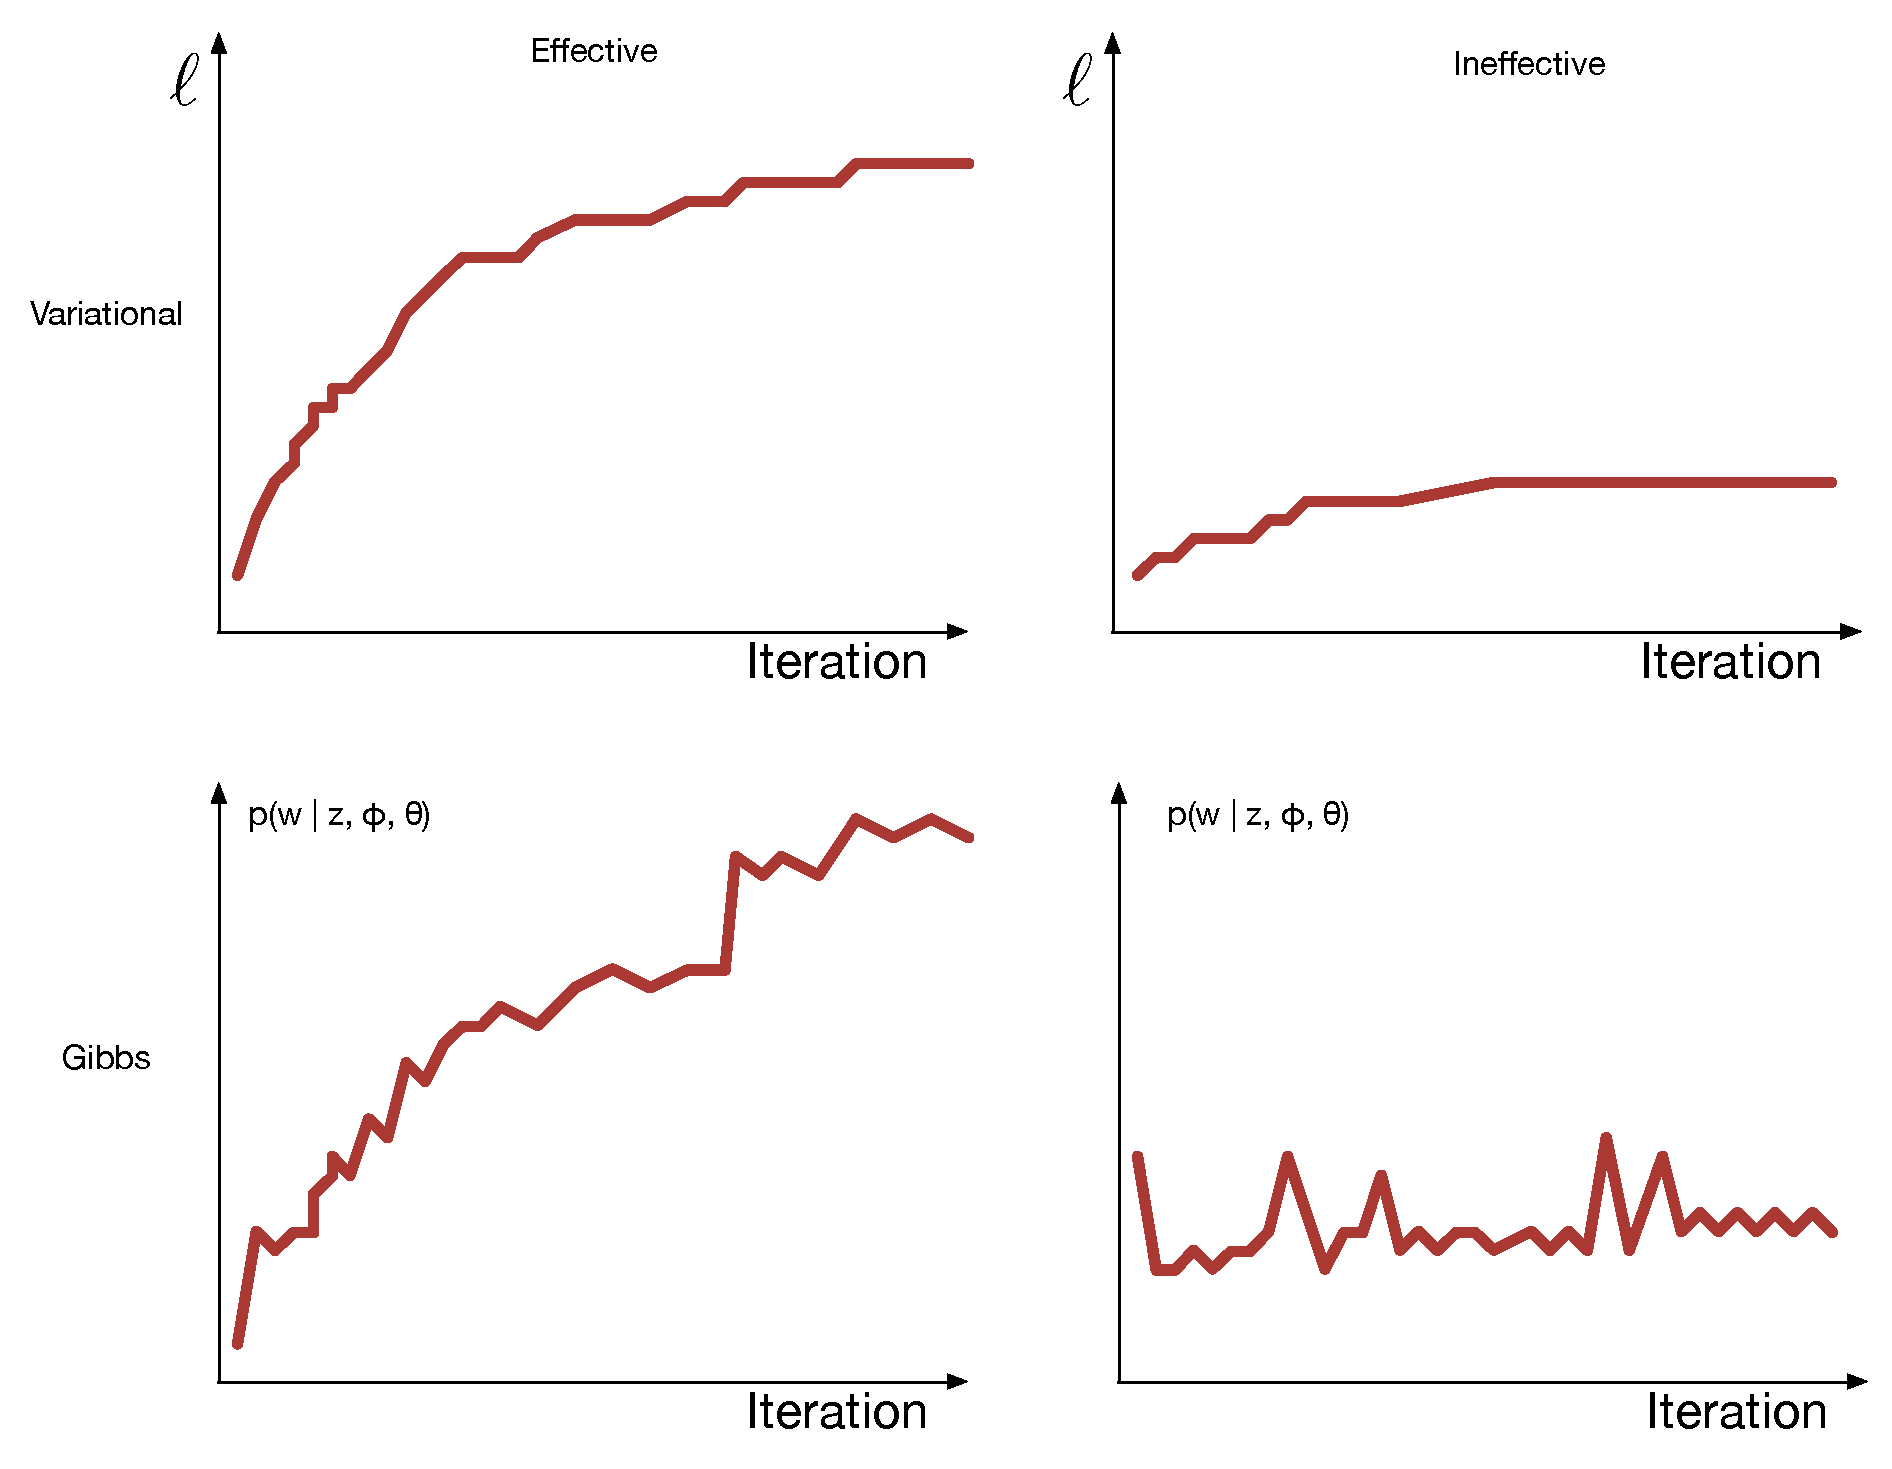
\includegraphics[width=.7\linewidth]{figures/objective_functions}

  \caption{Monitoring the objective function is an important component
  of diagnosing whether inference is working correctly.  Correct
  variational inference should increase monotonically while Gibbs
  sampling can decrease slightly.  However, in both cases, the
  objective function should increase dramatically over time.  If the
  objective is flat, it may mean that there are issues design choices
  in your inference algorithm.  Note: the
  scales for variational inference and Gibbs sampling are not
  comparable.}
  \label{fig:objective_func}
\end{figure}

Often a fully-factored variational distribution is a good choice.
After implementing a fully-factorized variational distribution, a
researcher should carefully monitor the objective function
(Equation~\ref{eq:obj}).  Ideally it will quickly increase and reach a
stable (local) optimum (Figure~\ref{fig:objective_func}, left).
However, if it does not (Figure~\ref{fig:objective_func}, right), then
it could be that there are coupled variables that are not well served
by the variational distribution.

Coupled variables need to change together, and a fully-factorized
distribution forces them to change in sequence.  For example, let's
say that $x=0$ and $y=0$ and that they are highly correlated, but a
higher probability setting is for $x=1$ and $y=1$.  Coordinate ascent
optimization with mean field will want to change $x$ or $y$
individually when they must move together.

To fully model the interaction between the two variables, we can model
$x$ and $y$ jointly in the variational distribution.  Instead of
independent distributions $q(x)q(y)$, the variational distribution
becomes $q(x,y)$ (as appropriate for whatever form those variables take).

\subsection{Gibbs Sampling}

Gibbs sampling (as discussed at a high level in Chapter~\ref{ch:intro}) finds
latent variables by randomly sampling an assignment of each random
variable conditioned on all of the other random variables.

Thus, after creating your model, you need to compute the conditional
distribution of each random variable conditioned on all of the
others.  For example, the conditional distribution of the topic
assignment of a word $z_{d,n}$ is
\begin{equation}
p(z_{d,n} \g z_{d, 1} \dots z_{d, n-1}, z_{d, n+1}, \dots z_{d, N_d},
\theta, \phi) = \frac{z_{d, 1} \dots z_{d, N_d}, \theta, \phi)}{ p(z_{d, 1} \dots z_{d, n-1}, z_{d, n+1}, \dots z_{d, N_d},
\theta, \phi)},
\label{eq:gibbs_conditional}
\end{equation}
which simplifies into Equation~\ref{eq:sampling}.

Deriving conditional distributions is often simpler than expanding
variational expectations.  For a step-by-step tutorial on deriving
Gibbs sampling for probabilistic models, see \citet{hardisty-10}.

\paragraph{Marginalization and Joint Variables}

Just like there is some art in deciding which variables to join
together in a joint distribution for variational inference, in Gibbs
sampling, you need to decide which variables to sample jointly and
which variables to marginalize.

Jointly sampling variables solves the same problem as merging
variables into the same variational distribution above.  Instead of
sampling $x$ conditioned on all other variables and then sampling $y$,
$x$ and $y$ are sampled \emph{at the same time} from a distribution
that conditions $x$ and $y$ on all of the other variables.

\section{Debugging and Validation}

Now that you have implemented inference for your topic model, how do
you know if it's working as intended?

\subsection{Synthetic Data}

Because most topic models have a generative story, we can
\emph{generate} data.  This means running the probabilistic story of
the model forward to generate data.  For example, for \abr{lda},
sample a topic distribution for each document and a type distribution
for each topic from Dirichlet distribution.  Such a dataset is often
called a \emph{synthetic} dataset.

If you create a dataset this way, the latent variables are no longer
latent.  You know \emph{exactly} what they are.  If you run inference
on these data you should be able to recreate the unmasked latent
variables you generated.  If your inference algorithm does not come
close, there is likely a problem with your inference procedure.

However, topic models can be tricky.  Topic~7 in your synthetic data
may correspond to Topic~4 that you discovered in inference.  That is
not a problem as the topic identifiers are arbitrary; thus, you will
have to match topics greedily or measure some other statistic to
compare your inferred variables with the true synthetic data.

Synthetic data is most valuable when it is close to the distribution of real data.
Toy problems can be a good sanity check, but provide at best a loose upper bound on our ability to model data that we care about.
Using {\em semi-synthetic} data can therefore be a good compromise.
In this setting, you train a model from real data, and then generate new documents from that model.
The resulting semi-synthetic corpus has many of the correct properties of natural documents, such as vocabulary size and sparsity, but is guaranteed to actually fit the proposed model.

\subsection{Updates}

For both variational inference and Gibbs sampling, the most important
step is updating the distribution for individual random variables.
Thus, you will want to take as many steps to ensure their accuracy as
possible.

For variational inference, each update of the variational parameters
increases the objective function (Equation~\ref{eq:obj}).  Thus, you can
check after every update of a variable's variational distribution
whether that objective has increased or not.  While not every update
will exactly increase the objective (due to numerical precision errors or
initialization), no update should dramatically \emph{decrease} the
objective.  If one does, you likely have a bug.

Gibbs sampling is stochastic, so it is more difficult to debug.  But
for both variational inference and Gibbs sampling, you should write
unit tests (worked out with pen and paper) to verify that your updates
reach the right answer given the same inputs.  Gibbs sampling's
randomness can be handled in a unit testing environment using stubs
that replace the random number generator (these stubs can also be
useful when you later want to generate results with different random
seeds, as discussed below).

\subsection{Baselines and Metrics}

Often you will want to compare your model to another model that either
has a similar structure or application.  This comparison can help you during
development.

For example, you may want to extend supervised \abr{lda} in some way
(Chapter~\ref{ch:css}).  Fortunately, \abr{slda} is a well-defined model and
has established performance on widely available datasets.

Thus, a reasonable development strategy would be to create a series of
models that take you from \abr{slda} to your final model (e.g., adding
one latent variable at a time), at each time comparing how well your
model does against \abr{slda}.  These comparisons do not just aid
development; they will also help document how important each of the
changes to the model are.

Comparisons between topic models can be difficult because implementations and algorithms can vary so much.
It is often unclear, for example, whether an observed difference is due to one model being better than another or to comparing Gibbs sampling to variational inference.
An excellent way to test a new algorithm for a complicated model is to find ways to implement simpler models in the same code.
For example, you can emulate an LDA model using an Author-Topic model \cite{rosen-zvi-04} by assigning each document its own ``author''.

A standard metric to report for topic models is their perplexity or
held-out likelihood.  This value is the probability of held-out data given
the settings of the model.  \citet{wallach-09a} detail a 
method for estimating perplexity in topic models given a Gibbs sampling algorithm (which is
beyond the scope of this survey).

However, perplexity is often not what you care about for your
application of topic models. For example, if you developing a variant
of \abr{slda}, you likely care about prediction accuracy.  Thus, as
you are slowly building out your \abr{slda} variant, you should report
prediction performance as well.

\section{Communicating Your Model}

After building a model, implementing inference, and applying it to
data, the next exciting step is to tell the world.  While one must
obviously provide motivation for a new model and describe the
technical details, one component of communicating a model that is
often overlooked is the interplay between these two facets of
describing a model.

The application should not just stand alongside the modeling goal; it
should be tightly integrated in the probabilistic story.  Rather than
simply listing the steps of the generative process, the generative
process should be described with evocative variable names.  For
example, if your model attempts to capture political polarization,
then you may call a discrete variable ``polarization $\pi$'' to
make it clear where in the model this aspect will be modeled.

However, simply naming a variable does not make it so.  You will also
need to provide qualitative evidence that will convince a skeptical
reader that your model is doing what you promised.  This is possible
by providing overviews of your data at either the micro or macro
level.

At the macro level, you can show that your model is doing reasonable
things by showing the distribution over words given topics (or
whatever the analogous component is).  However, you should avoid the
temptation to cherry-pick topics.  It is better to select topics
randomly or---if you do cherry-pick---to also select ``bad'' topics
that show failure modes of your model.

While macro level cues can show the model finds good summaries, you
should also show individual documents and how they interact with
data.  For example, if your model attempts to show political
polarization, you can show polarized (or not) documents and show how
the latent variables in your models correctly capture those aspects of
the documents (or not; as with topics, it is important to show failure
modes as well).

In addition, you will also have quantitative metrics for your task.
This could be accuracy of prediction, precision at rank $K$, or
translation quality (Chapter~\ref{ch:mt}).  When reporting quantitative
results, it's important to remember the probabilistic foundations of
topic models: you are not learning one answer.  Regardless of the
inference, you are learning a \emph{distribution} over latent
variables given a dataset.

Thus, it is important to convey the inherent uncertainty in inference.
You should run inference multiple times with different random seeds
(Gibbs sampling) or random initializations (variational inference).
This allows you to report quantitative results with error bars to make
credible comparisons to other models: not only do you have a higher
score but you show that your higher score is not just the result of
chance.

\section{Conclusion}

In this chapter, we discussed the process for creating a new topic
model from scratch and how to communicate this process to the world.
While superficially different than our application-focused chapters,
most of the papers were created through this process of
model-building, inference, and evaluation.  Thus, this chapter helps
understand the process for building the models that we've discussed
through these chapters.

In the next chapter, we contemplate the future of topic models and how
topic models might fit into the broader computer and information
science research agenda.
